\section[SDL]{La bibliothèque SDL}

\subsection{SDL} %%%%%%%%%%%%%%%%%%%%%%%%%%%%%%%%%%%%%%%%%%%%
\begin{frame}
	\begin{center}
		\huge
		La bibliothèque SDL
	\end{center}
\end{frame}

\begin{frame}
	\frametitle{Le principe actif SDL}
	\begin{center}
		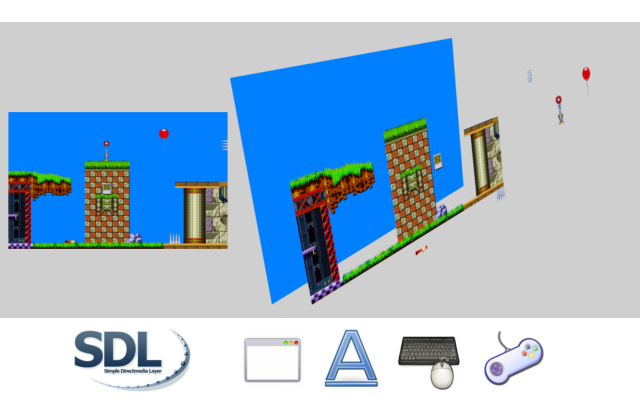
\includegraphics[width=9cm]{pics/sdlSurfaces.png}
	\end{center}
\end{frame}

\begin{frame}[fragile]
	\frametitle{Les modules SDL}
	\begin{columns}
		\begin{column}{3cm}
			\begin{itemize}
				\item Sdl
				\item Sdlwm
				\item Sdlvideo
				\item Sdltime
				\item Sdlevent
			\end{itemize}
		\end{column}
		\begin{column}{3cm}
			\begin{itemize}
				\item Sdlttf
				\item Sdlloader
				\item Sdlmixer
				\item Sdlgfx
			\end{itemize}
		\end{column}
	\end{columns}
\end{frame}

\subsection{Introduction à SDL} %%%%%%%%%%%%%%%%%%%%%%%%%%%%%%%%%%%%%%%%%%%%%%%
\begin{frame}[fragile]
	\frametitle{Initialisation de SDL}
	\begin{columns}
		\begin{column}{5cm}
			\begin{block}{L'initialisation de base}
				\lstset{basicstyle=\small}
				\begin{lstlisting}
  Sdl.init [`EVERYTHING]
				\end{lstlisting}
			\end{block}
			\begin{block}{L'initialisation et ouverture d'une fenêtre}
				\lstset{basicstyle=\small}
				\begin{lstlisting}
  Sdl.init [`EVERYTHING]

  let screen =
   Sdlvideo.set_video_mode
   ~w ~h ~bpp [`HWSURFACE]
				\end{lstlisting}
			\end{block}
			\begin{block}{Quitter Sdl}
				\lstset{basicstyle=\small}
				\begin{lstlisting}
  Sdl.quit ()
				\end{lstlisting}
			\end{block}
		\end{column}
		\begin{column}{3.3cm}
			\begin{block}{Types d'initialisation}
				\begin{itemize}
					\item `AUDIO
					\item `CDROM
					\item `JOYSTICK
					\item `TIMER
					\item `VIDEO
				\end{itemize}
				\begin{itemize}
					\item `EVERYTHING
				\end{itemize}
			\end{block}
		\end{column}
	\end{columns}
\end{frame}

\subsection{L'affichage bas niveau} %%%%%%%%%%%%%%%%%%%%%%%%%%%%%%%%%%%%%%%%%%%
\begin{frame}[fragile]
	\frametitle{Quelques mots sur les surfaces}
	\framesubtitle{Type de la surface}
	\begin{columns}
		\begin{column}{5.2cm}
			\begin{block}{Caractéristiques}
				\lstset{basicstyle=\small}
				\begin{lstlisting}
type surface_info = {
  flags : surface_flags list;
  w : int;
  h : int;
  pitch : int;
  clip_rect : rect;
  refcount : int;
}
				\end{lstlisting}
			\end{block}
		\end{column}
		\begin{column}{3.6cm}
			\begin{block}{Types}
				\begin{itemize}
					\item `FULLSCREEN
					\item `HWSURFACE
					\item `OPENGL
					\item `SWSURFACE
					\item `SRCALPHA
					\item `RESIZABLE
					\item `SRCCOLORKEY
					\item `DOUBLEBUF
				\end{itemize}
			\end{block}
		\end{column}
	\end{columns}
\end{frame}


\begin{frame}
	\frametitle{Quelques mots sur les surfaces}
	\framesubtitle{La surface de type \textit{Double Buffer}}
	\begin{center}
		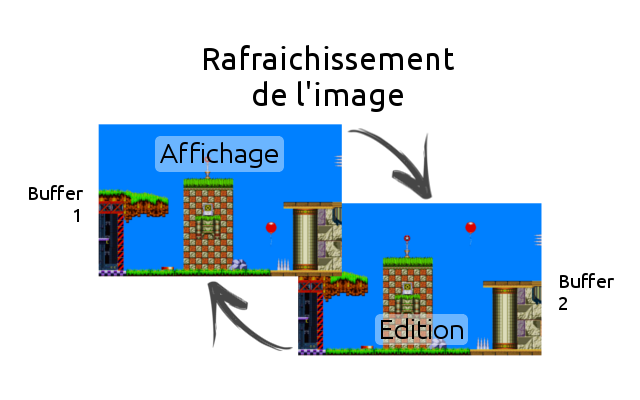
\includegraphics[width=9cm]{pics/doubleBuffer.png}
	\end{center}
\end{frame}

\begin{frame}[fragile]
	\frametitle{Quelques mots sur les surfaces}
	\framesubtitle{Le type rect}
	\begin{center}\begin{minipage}{0.4\textwidth}
		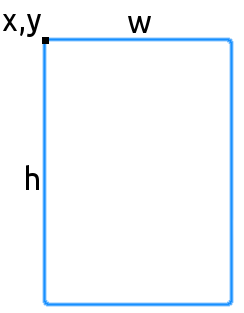
\includegraphics[width=3cm]{pics/rect.png}
	\end{minipage}
	\begin{minipage}{0.4\textwidth}
		\begin{block}{Position et dimension}
			\lstset{basicstyle=\footnotesize}
			\begin{lstlisting}
  type rect = {
    mutable r_x : int;
    mutable r_y : int;
    mutable r_w : int;
    mutable r_h : int;
  }
			\end{lstlisting}
		\end{block}
	\end{minipage}\end{center}
	\begin{block}{Fonctions liées}
		\lstset{basicstyle=\footnotesize}
		\begin{lstlisting}
  val rect : x:int -> y:int -> w:int -> h:int -> rect

  val surface_dims : surface -> int * int * int
		\end{lstlisting}
	\end{block}
\end{frame}

\begin{frame}[fragile]
	\frametitle{Le chargement d'image}
	\begin{block}{Charger/Sauvegarder une image .bmp}
		\begin{lstlisting}
  val load_BMP : string -> surface

  val save_BMP : surface -> string -> unit
		\end{lstlisting}
	\end{block}
	\begin{block}{Charger une image .jpeg .png .tiff}
		\begin{lstlisting}
  val Sdlloader.load_image : string -> surface

		\end{lstlisting}
	\end{block}
\end{frame}

\begin{frame}
	\frametitle{Les pixels}
	\begin{center}
		
\includegraphics[width=9cm]{pics/Joconde-pixel.jpg}
	\end{center}
\end{frame}

\begin{frame}[fragile]
	\frametitle{Les pixels}
	\framesubtitle{La couleur}
	\begin{block}{Types}
		\textit{La couleur peut être sous la forme d'un color ou d'un int32.}
		\begin{lstlisting}
  type color = int * int * int
  let c = ((255,255,255):color)
		\end{lstlisting}
	\end{block}
	\begin{block}{Fonctions de conversion}
		\begin{lstlisting}
  val map_RGB : surface -> ?alpha:int ->
    color -> int32
  val get_RGB : surface -> int32 -> color
  val get_RGBA : surface -> int32 ->
    color * int
		\end{lstlisting}
	\end{block}
\end{frame}

\begin{frame}[fragile]
	\frametitle{Les pixels}
	\framesubtitle{\og{}Bon ! Quand est-ce qu'on manipule des pixels ?\fg}
	\begin{block}{Verrouillage de la surface}
		\begin{lstlisting}
  val lock : surface -> unit
  val unlock : surface -> unit
  val must_lock : surface -> bool
		\end{lstlisting}
	\end{block}
	\begin{block}{Modification de la surface}
		\begin{lstlisting}
  val get_pixel : surface -> x:int ->
    y:int -> int32

  val put_pixel : surface -> x:int ->
    y:int -> int32 -> unit
		\end{lstlisting}
		\textit{Existe aussi en version prenant le type color au lieu de int32. Pour cela ajouter le suffixe \_color à la fonction.}
	\end{block}
\end{frame}

\begin{frame}[fragile]
	\frametitle{\og{}Merge Down !\fg}
	\begin{center}
		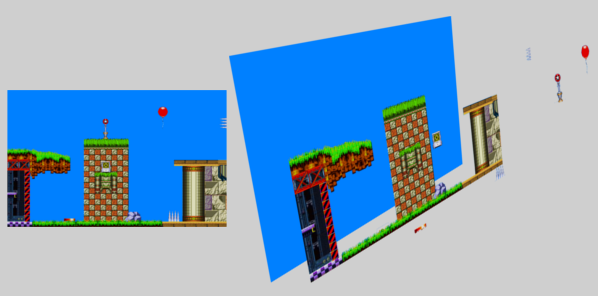
\includegraphics[width=3.6cm]{pics/surfacesMerge.png}
	\end{center}
	\begin{block}{Écraser/Créer un fond de couleur}
		\begin{lstlisting}
  val fill_rect : ?rect:rect -> surface ->
    int32 -> unit
		\end{lstlisting}
	\end{block}
	\begin{block}{Coller une surface sur une autre}
		\begin{lstlisting}
  val blit_surface : src:surface ->
    ?src_rect:rect ->  dst:surface ->
    ?dst_rect:rect -> unit -> unit
		\end{lstlisting}
	\end{block}
\end{frame}

\begin{frame}[fragile]
	\frametitle{L'actualisation de l'affichage}
	\framesubtitle{Surface Utilisateur}
	\begin{center}
		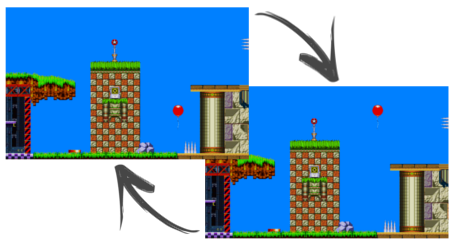
\includegraphics[width=2.4cm]{pics/doubleBufferScreen.png}
	\end{center}
	\begin{block}{La surface \og{}Fenêtre utilisateur\fg}
		\begin{lstlisting}
  val set_video_mode : w:int ->
    h:int -> ?bpp:int ->
    video_flag list -> surface
  val get_video_surface : unit ->
    surface
		\end{lstlisting}
	\end{block}
	
\end{frame}

\begin{frame}[fragile]
	\frametitle{L'actualisation de l'affichage}
	\framesubtitle{Rafraîchissement de la surface utilisateur}
	\begin{center}
		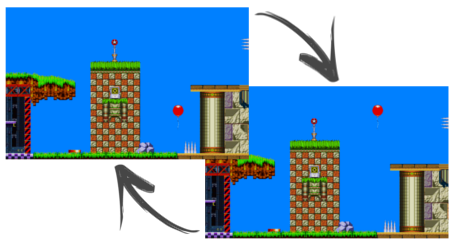
\includegraphics[width=2.4cm]{pics/doubleBufferScreen.png}
	\end{center}
	\begin{block}{Fonction de rafraîchissement}
		\begin{lstlisting}
  val update_rect : ?rect:rect ->
    surface -> unit
  val update_rects : rect list ->
    surface -> unit
		\end{lstlisting}
	\end{block}
	\begin{block}{Rafraîchissement pour un \textit{Double Buffer}}
		\begin{lstlisting}
  val flip : surface -> unit
		\end{lstlisting}
	\end{block}
\end{frame}

\begin{frame}[fragile]
	\frametitle{Créer des surfaces à partir de rien}
	\lstset{basicstyle=\footnotesize}
	\begin{lstlisting}
val create_RGB_surface_format : surface ->
  [ `ASYNCBLIT | `HWSURFACE | `SRCALPHA
  | `SRCCOLORKEY | `SWSURFACE ] list ->
  w:int -> h:int -> surface

val create_RGB_surface :
  [ `ASYNCBLIT | `HWSURFACE | `SRCALPHA
  | `SRCCOLORKEY | `SWSURFACE ] list ->
  w:int -> h:int -> bpp:int ->
  rmask:int32 -> gmask:int32 -> bmask:int32 ->
  amask:int32 -> surface
	\end{lstlisting}
\end{frame}

\subsection{La détection d'événement} %%%%%%%%%%%%%%%%%%%%%%%%%%%%%%%%%%%%%%%%%
\begin{frame}[fragile]
	\frametitle{Détecter et récupérer un événement}
	\begin{block}{Attendre l'utilisateur}
		\begin{lstlisting}
  val wait_event : unit -> event
		\end{lstlisting}
	\end{block}
	\begin{block}{Traiter la file des derniers événements}
		\begin{lstlisting}
  val poll : unit -> event option
		\end{lstlisting}
	\end{block}
\end{frame}

\begin{frame}[fragile]
	\frametitle{Les différents types d'événements}
	\lstset{basicstyle=\small}
	\begin{lstlisting}
type event =
| ACTIVE of active_event
| KEYDOWN of keyboard_event
| KEYUP of keyboard_event
| MOUSEMOTION of mousemotion_event
| MOUSEBUTTONDOWN of mousebutton_event
| MOUSEBUTTONUP of mousebutton_event
| JOYAXISMOTION of joyaxis_event
| JOYBALLMOTION of joyball_event
| JOYHATMOTION of joyhat_event
| JOYBUTTONDOWN of joybutton_event
| JOYBUTTONUP of joybutton_event
| QUIT
| SYSWM
| VIDEORESIZE of int * int
| VIDEOEXPOSE
| USER of int
	\end{lstlisting}
\end{frame}

\begin{frame}[fragile]
	\frametitle{Sous-événement Clavier/Souris}
	\lstset{basicstyle=\scriptsize}
	\begin{block}{Clavier}
		\begin{lstlisting}
  type keyboard_event = {
    ke_which : int;
    ke_state : switch_state;
    keysym : Sdlkey.t;
    keymod : Sdlkey.mod_state;
    keycode : char;
    unicode : int;
  }
		\end{lstlisting}
	\end{block}
	\begin{block}{Souris}
		\begin{minipage}{0.47\textwidth}
			\begin{lstlisting}
  type mousemotion_event = {
    mme_which : int;
    mme_state :
      Sdlmouse.button list;
    mme_x : int;
    mme_y : int;
    mme_xrel : int;
    mme_yrel : int;
  }
			\end{lstlisting}
		\end{minipage}
		\begin{minipage}{0.4\textwidth}
			\begin{lstlisting}
  type mousebutton_event = {
    mbe_which : int;
    mbe_button :
      Sdlmouse.button;
    mbe_state : switch_state;
    mbe_x : int;
    mbe_y : int;
  }
			\end{lstlisting}
		\end{minipage}
	\end{block}
\end{frame}

\subsection{Une boucle Sdl classique} %%%%%%%%%%%%%%%%%%%%%%%%%%%%%%%%%%%%%%%%%
\begin{frame}[fragile]
	\frametitle{Actualisation d'une application SDL simple}
	\large
	\begin{itemize}
		\item Boucle principale
		\item Gestion des événements
		\item Actualisation de l'écran
	\end{itemize}
\end{frame}

\begin{frame}[fragile]
	\frametitle{Boucle Principale}
	\begin{lstlisting}
let update () =
  let ticks = (*17ms -> 60fps *)
    17 + Sdltimer.get_ticks ()
  in
  updateEvent();
  updateDisplay();
  while (Sdltimer.get_ticks ()) <= ticks do
    () done
	\end{lstlisting}
\end{frame}

\begin{frame}[fragile]
	\frametitle{Gestion des événements}
	\begin{lstlisting}
let updateEvent () =
  match Sdlevent.poll () with
  | None -> ()
  | Some (Sdlevent.KEYDOWN key) ->
    keyDownManager key
  | Some (Sdlevent.MOUSEBUTTONDOWN button) ->
    buttonDownManager button
  | Some Sdlevent.QUIT -> Sdl.quit ()
  | _ -> ()
	\end{lstlisting}
\end{frame}

\begin{frame}[fragile]
	\frametitle{Modification et déplacement des élements visuels}
	\lstset{basicstyle=\scriptsize}
	\begin{lstlisting}
val blit_surface : src:surface -> ?src_rect:rect ->
  dst:surface -> ?dst_rect:rect -> unit -> unit
	\end{lstlisting}
	\textit{Soit displayData une file de fonctions Sdlvideo.blit\_surface dont tous les paramètres sont renseignés sauf le unit final}
	\lstset{basicstyle=\normalsize}
	\begin{lstlisting}
let updateDisplay () =
  while not (is_empty displayData) do
    (take displayData) ()
  done
	\end{lstlisting}
\end{frame}
